\section{What correlation can and cannot identify}
\label{sec:identification}

Fix $n\ge2$ items with true rating distributions $P_i$ on $\{0,\dots,K-1\}$, item means $t_i$, forecasts $q_i$ and forecast means $m_i$.
Pearson correlation across items is $\rho(m,t)=\sum_i(m_i-\bar m)(t_i-\bar t)/(n\,s_m s_t)$ and is undefined when either vector is constant.
All statements below are proved in \appref{app:proofs}; they restate the identification preprint~\citep{miranda2026correlation} with the cross-entropy (CE), ranked probability score (RPS) and Pearson definitions of Section~\ref{sec:setting}.

\begin{proposition}[Pearson sees means up to a positive affine map]
\label{prop:affine}
For nonconstant $m$ and $t$, forecasts with equal item means have equal correlation, $\rho(a\mathbf 1+bm,t)=\rho(m,t)$ for every $a\in\mathbb R$ and $b>0$, and $\rho(m,t)=1$ if and only if $m=a\mathbf 1+bt$ for some $a\in\mathbb R$, $b>0$.
\end{proposition}

The statement concerns the output, not the model.
A neural judge may map inputs to means by any nonlinear function and still reach $\rho=1$; Pearson measures the linear association between predicted and human ratings, and does not make the judge linear.

\begin{proposition}[Unidentified directions]
\label{prop:dimension}
For $K=2$ a forecast is fixed by its mean, so correlation one leaves only the level $a$ and scale $b$.
For $K\ge3$ the distributions with a fixed interior mean form a set of dimension $K-2$, and the all-positive set of forecasts with correlation one has dimension $n(K-2)+2$.
\end{proposition}

Binary ratings therefore remove the shape ambiguity and keep the level and scale ambiguity.
For $K=2$ and correlation-one means $m_i=a+bt_i$, the excess expected RPS is $n^{-1}\sum_i(a+(b-1)t_i)^2$, which is zero only at $a=0$, $b=1$.
Three or more categories add $K-2$ free shape directions per item.

\begin{proposition}[What each objective identifies]
\label{prop:losses}
(i) Mean squared error satisfies $\E[(a-R)^2\mid x]=(a-t(x))^2+\Var(R\mid x)$, so it identifies the conditional mean and nothing else.
(ii) $\CE(P,q)=H(P)+\KL(P\|q)$, so CE is uniquely minimized by $q=P$.
(iii) With $d_k=F_P(k)-F_q(k)$, $\bar d$ their average and $m_q,m_P$ the two means, the excess expected RPS is
\begin{equation}
\mathcal E_P(q)=\frac{(m_q-m_P)^2}{(K-1)^2}+\frac1{K-1}\sum_{k=0}^{K-2}(d_k-\bar d)^2 ,
\label{eq:rps-decomp}
\end{equation}
which vanishes only at $q=P$, and $|m_q-m_P|\le(K-1)\TVD(P,q)$.
\end{proposition}

Equation~\eqref{eq:rps-decomp} shows what RPS adds to a mean: the first term is the mean error, the second is everything else in the cumulative distribution, and it is the only term that remains when the means agree.
Total variation distance to the true distribution is zero only at $q=P$ but is not a proper score for individual ratings (\appref{app:proofs}), which is why we report it as a diagnostic.

\begin{proposition}[CE controls every bounded moment]
\label{prop:moments}
For $m_j(q,x)=\E_q[(R/(K-1))^j\mid x]$ and every integer $j\ge1$,
\[
\E_X\bigl[(m_j(q,X)-m_j(p,X))^2\bigr]\le\tfrac12\bigl(\CE(q)-\CE(p)\bigr).
\]
\end{proposition}

A model that lowers population CE toward its minimum therefore recovers the mean, variance, skewness and every other moment at the same time; Pearson correlation constrains only the first.
The converse is the content of the next result.

\begin{proposition}[Means alone cannot recover shape]
\label{prop:lower}
Let $P_0\ne P_1$ have equal means and $d=\TVD(P_0,P_1)$, and let a rule see only the mean and output $q$.
Then $\max_j\TVD(P_j,q)\ge d/2$, $\max_j\KL(P_j\|q)\ge d^2/2$ and $\tfrac12(\mathcal E_{P_0}(q)+\mathcal E_{P_1}(q))\ge D(P_0,P_1)/(4(K-1))$ with $D=\sum_k(F_{P_0}(k)-F_{P_1}(k))^2$.
\end{proposition}

\paragraph{Gradients.}
For $q_i=\mathrm{softmax}(u_i)$, $\partial\rho/\partial u_i(r)=g_iq_i(r)(r-m_i)$ with $g_i=(\zeta_i-\rho z_i)/(ns_m)$, while $\partial\sum_j\CE(P_j,q_j)/\partial u_i(r)=q_i(r)-P_i(r)$.
A shape output that is parameterized apart from the mean receives no direct correlation gradient; with shared parameters, correlation can still change the shape indirectly, which is why the identification statements do not predict how a trained judge behaves and we test it below.

\begin{figure*}[t]
\centering
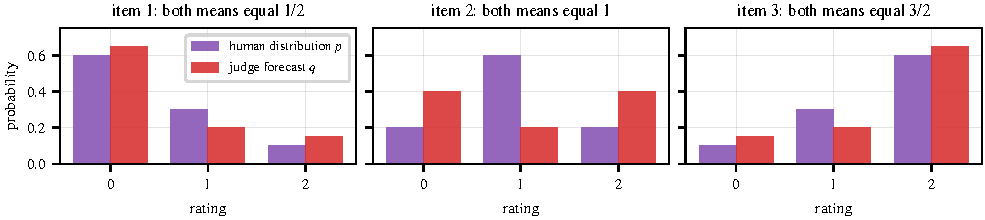
\includegraphics[width=\textwidth]{figures/fig_counterexample.pdf}
\caption{\textbf{Exact counterexample ($K=3$ ratings 0, 1, 2; $n=3$ items).}
Purple bars: the human rating distribution $P_i$; red bars: the judge's forecast $q_i$.
Both have the same item means ($\tfrac12$, $1$, $\tfrac32$), so the Pearson correlation between forecast means and human means is exactly 1.
The forecast is nevertheless wrong in shape: mean total variation distance to the human distributions $0.20$ (lower is better, range 0--1), excess RPS $3/200=0.015$ (range 0--1, lower is better), and cross-entropy $1.065$ nats against $0.915$ nats for the true distributions (CE of $P$ against itself is its entropy).
Every number is exact; no ratings are sampled.
\textbf{Takeaway:} correlation one does not imply the right distribution, and CE and RPS separate the two forecasts.}
\label{fig:counterexample}
\end{figure*}

\paragraph{An exact example.}
\Cref{fig:counterexample} gives three items on three ratings with human distributions $P_1=(0.6,0.3,0.1)$, $P_2=(0.2,0.6,0.2)$ and $P_3=(0.1,0.3,0.6)$.
The forecast matches every item mean, so $\rho=1$, yet its rating variances are $11/20$, $4/5$ and $11/20$ against $9/20$, $2/5$ and $9/20$ for the humans (derivation and table in \appref{app:proofs}; a committed script reproduces it in \expref{27}).

\paragraph{What this does not say.}
The propositions concern the set of population optima.
They do not say that every correlation-trained judge lands on a wrong shape; initialization, regularization, tie rules and model restrictions can select the true distribution from the optimum set, and a nonlinear judge may recover it from features.
They also give no universal break-even sample size.
The heuristic $N\approx P/(2B)$, from the regular asymptotic excess CE $P/(2N)$ of a $P$-parameter maximum-likelihood fit against a fixed excess CE $B$ of the competitor, holds only in CE nats under its asymptotic assumptions and cannot take an RPS gap in place of $B$.
How many ratings a cross-entropy fit needs is therefore an empirical question, and the rest of the memo measures it.
